\section{Fundamentação e trabalhos relacionados}
\label{sec:relacionados}
A literatura é organizada em três eixos: detecção de anomalias; atividade ilícita, \textit{front-running} e MEV na Ethereum; e avaliação sob desbalanceamento e mudanças temporais. A Figura~\ref{fig:revisao-literatura} apresenta o fluxo de leitura e síntese, que compara unidades de análise, atributos, rótulos e objetivos dos estudos.

\begin{figure}[!t]
\centering
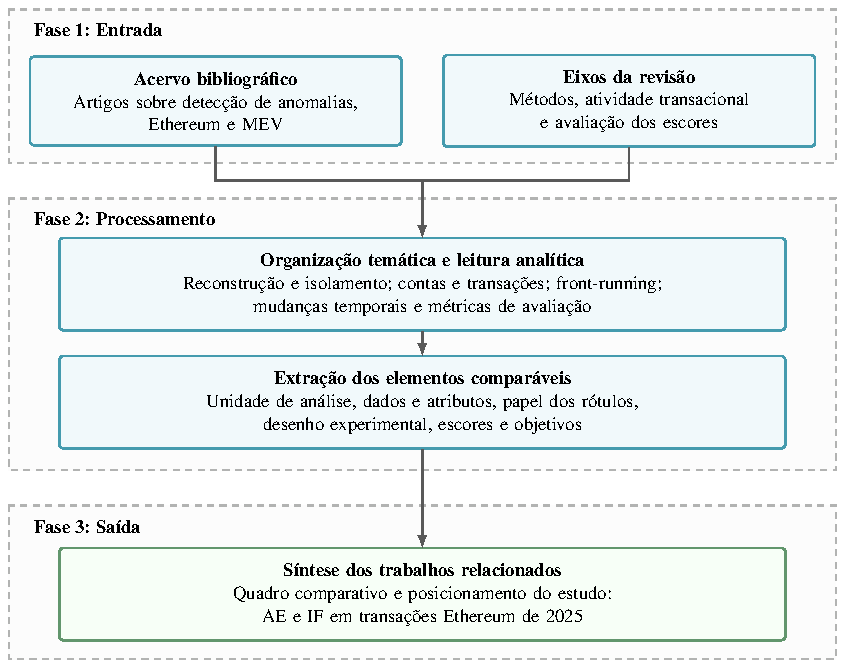
\includegraphics[width=.70\linewidth]{imagens/fluxograma-literatura.pdf}
\caption{Fluxograma de organização e análise da literatura utilizada nos trabalhos relacionados.}
\label{fig:revisao-literatura}
\end{figure}

\subsection{Reconstrução e isolamento na detecção de anomalias}
Sakurada e Yairi \cite{Sakurada2014} investigam autoencoders para detecção de anomalias por redução não linear de dimensionalidade, em dados artificiais e telemetria. O erro de reconstrução mede o afastamento de uma observação da representação aprendida e fundamenta o escore transacional do AE neste estudo.

Liu et al.\ \cite{Liu2008} propõem o Isolation Forest, que constrói árvores aleatórias sobre subamostras e associa caminhos médios curtos a observações mais facilmente isoladas. Reconstrução e isolamento produzem escores com escalas distintas; sua aplicação à mesma população permite comparar conjuntos priorizados pelos dois mecanismos.

\subsection{Contas, transações e padrões de MEV na Ethereum}
Farrugia et al.\ \cite{Farrugia2020} classificam contas Ethereum com XGBoost, utilizando 42 atributos e 4.681 contas, das quais 2.179 rotuladas como ilícitas. A agregação do histórico caracteriza a conta; a unidade transacional adotada aqui permite examinar operações individuais de um mesmo remetente.

Podgorelec et al.\ \cite{Podgorelec2020} incorporam detecção personalizada de anomalias à assinatura automatizada de transações Ethereum. O perfil individual orienta uma decisão anterior à assinatura, enquanto nosso protocolo examina operações executadas e seu contexto intrabloco.

Daian et al.\ \cite{Daian2020} relacionam bots de arbitragem e \textit{priority gas auctions} à extração de valor pela ordenação transacional. Eskandari, Moosavi e Clark \cite{Eskandari2020} sistematizam \textit{front-running} em deslocamento, inserção e supressão, padrões investigados empiricamente na Ethereum por Torres et al.\ \cite{Torres2021}. Esses trabalhos fornecem o contexto econômico e estrutural para interpretar operações priorizadas pelos detectores.

Heimbach et al.\ \cite{Heimbach2023} analisam a \textit{proposer-builder separation}, distinguindo construção e proposição dos blocos. Essa organização contextualiza a interpretação conjunta de taxas, posição e contexto transacional na atividade associada a MEV.

Zhang et al.\ \cite{Zhang2024FRAD} apresentam o FRAD, com classificação ternária de deslocamento, inserção e supressão. Li et al.\ \cite{Li2024Geth} integram ao Geth a detecção de ataques \textit{sandwich} em tempo próximo ao real. Enquanto essas abordagens focalizam categorias de ataques, comparamos escores de anomalia em toda a população transacional selecionada (Tabela~\ref{tab:comparacao-trabalhos}).

\begin{table}[htbp]
\centering\small
\caption{Posicionamento do estudo em relação às abordagens aplicadas à Ethereum.}
\label{tab:comparacao-trabalhos}
\renewcommand{\arraystretch}{1.12}
\begin{tabularx}{\linewidth}{@{}>{\raggedright\arraybackslash}p{4cm}>{\raggedright\arraybackslash}p{2.6cm}>{\raggedright\arraybackslash}X@{}}
\toprule
Trabalho & Unidade ou foco & Abordagem e relação com este estudo \\
\midrule
\cite{Farrugia2020} & Contas ilícitas & Classificação supervisionada por atributos agregados de contas e histórico. \\
\cite{Podgorelec2020} & Assinatura de transações & Detecção personalizada associada à decisão de assinatura. \\
\cite{Torres2021} & Padrões de front-running & Identificação empírica de inserção, deslocamento e supressão. \\
\cite{Zhang2024FRAD} & Categorias de front-running & Classificação ternária das categorias de ataque. \\
\cite{Li2024Geth} & Ataques sandwich & Detecção integrada ao cliente Geth. \\
Este artigo & Transações individuais & AE e IF com parâmetros pré-selecionados, avaliação temporal, concordância e associação MEV. \\
\bottomrule
\end{tabularx}
\end{table}


\subsection{Avaliação de escores e mudanças temporais}
Gama et al.\ \cite{Gama2014} discutem a adaptação a \textit{concept drift}, incluindo mudanças na relação entre entradas e alvos. Aqui, acompanhamos mudanças marginais de atributos e escores, mantendo os limiares congelados para observar sua relação com a evolução das sinalizações.

Saito e Rehmsmeier \cite{Saito2015} discutem ROC e Precision-Recall em populações desbalanceadas. Precision caracteriza a composição do conjunto sinalizado, e recall, a recuperação da referência positiva. Combinamos ROC-AUC, AP e concentração no topo do ranking para distinguir ordenação global, cobertura e volume de investigação.

Em síntese, reconstrução e isolamento fundamentam os detectores; os estudos de contas e transações distinguem unidades de análise e supervisão; e a literatura de MEV caracteriza padrões de interesse. Este artigo cruza esses eixos em uma comparação temporal de AE e IF com atributos comuns e parâmetros preselecionados. A decomposição da concordância quantifica a contribuição de cada método; ROC, Precision-Recall e associação histórica a bots MEV permitem relacionar essa contribuição às prioridades de investigação. Essa comparação constitui a base para uma futura avaliação semântica dos padrões priorizados.
